\section{Electrical Potential Difference}
\begin{definition}
    [Electrical Potential Difference] The change in the electrical potential between two points, and uses the symbol $\Delta V$
\end{definition}

\subsubsection{Formula}
Assume a charge q goes from a location where the electrical potential is $V_1$ to a location where the electrical potential is $V_2$
\begin{figure}[!h]
    \centering
    \includegraphics[width=0.5\textwidth]{pictures/4.5.1.png}
\end{figure}

Electrical Potential Energy of $q$\\

\begin{paracol}{2}
    \begin{leftcolumn}
        Loaction 1:\\

        $E_{E1} = q \times V_1$
    \end{leftcolumn}
    \begin{rightcolumn}
        Location 2:\\

        $E_{E2} = q \times V_2$
    \end{rightcolumn}
\end{paracol}

\begin{gather}
    \Delta E_E = E_{E2} - E_{E1} \nonumber \\
    \Delta E_E = q \times V_2 - q \times V_1  \nonumber \\
    \Delta E_E = q \times \Delta V
\end{gather}
\begin{remark}
    When use this formula, sub in all the signs!
\end{remark}

\begin{theorem}
    Assume we have two charges, $q_A$ (which is positive) and $q_B$(which is negative), the total electrical potential at a point in between $q_A$ and $q_B$ will be $V_A + V_B$\\

    If $\left| q_A \right| = \left| q_B\right|$ and $q_B = -q_A$, the electrical potential at the midpoint in between these two charges is 0.

    \begin{gather*}
        \lim_{\text{position} \rightarrow q_A} V = \infty\\
        \lim_{\text{position} \rightarrow q_B} V = -\infty\\
        \lim_{\text{position} \rightarrow \text{midpoint}} V = 0\\
    \end{gather*}
\end{theorem}
\noindent\hrulefill

A graph of the electrical potential would look like:
\begin{center}

\tikzset{every picture/.style={line width=0.75pt}} %set default line width to 0.75pt        

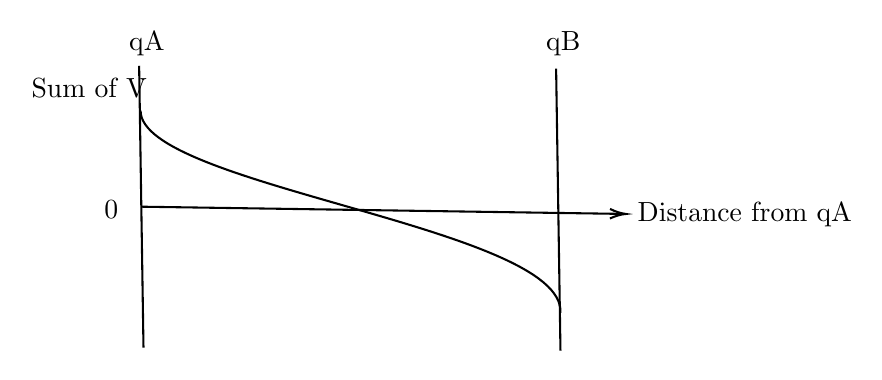
\begin{tikzpicture}[x=0.75pt,y=0.75pt,yscale=-0.7,xscale=0.7]
%uncomment if require: \path (0,300); %set diagram left start at 0, and has height of 300

%Straight Lines [id:da7110876361925111] 
\draw    (140.5,156.5) -- (472,161.47) ;
\draw [shift={(474,161.5)}, rotate = 180.86] [color={rgb, 255:red, 0; green, 0; blue, 0 }  ][line width=0.75]    (10.93,-3.29) .. controls (6.95,-1.4) and (3.31,-0.3) .. (0,0) .. controls (3.31,0.3) and (6.95,1.4) .. (10.93,3.29)   ;
%Straight Lines [id:da47576410206151465] 
\draw    (139,59.5) -- (142,253.5) ;
%Curve Lines [id:da8429044773147503] 
\draw    (140,90.5) .. controls (140,142.5) and (432,170.5) .. (429,229.5) ;
%Straight Lines [id:da49115835939959473] 
\draw    (426,61.5) -- (429,255.5) ;

% Text Node
\draw (63,66) node [anchor=north west][inner sep=0.65pt]   [align=left] {Sum of V};
% Text Node
\draw (480,151) node [anchor=north west][inner sep=0.75pt]   [align=left] {Distance from qA};
% Text Node
\draw (130,34) node [anchor=north west][inner sep=0.75pt]   [align=left] {qA};
% Text Node
\draw (417,34) node [anchor=north west][inner sep=0.75pt]   [align=left] {qB};
% Text Node
\draw (113,150) node [anchor=north west][inner sep=0.75pt]   [align=left] {0};


\end{tikzpicture}
\end{center}

If we put a new charge at the midpoint $q_A$ and $q_B$, we will find that $V = 0$ and $E_E = 0$. However, the charge would still move. To understand what will happen to this charge, we need to look at the energy gradient
\\

Roll Down!

\begin{remark}
    About \textit{Energy Gradient}, please follow teacher's note!
\end{remark}